\documentclass[11pt]{article}
\usepackage{fullpage}
\usepackage{graphicx}

\title{CS63 Fall 2019\\Lab 7: Deep Q-Learning}
\author{Ankur Malik, Ibrahem Hassouna}
\date{April 7, 2022}

\begin{document}

\maketitle

\section{RL Problem}

% TODO Describe the RL problem: states, actions, rewards
States encapsulate the current stage of the game, task, or environment. The state tells the agent where it is, encoding different attributes specific to the present situation.
Actions are the moves agents make to go from one state to another.
Rewards are immediate and external to the agent (they are supplied by the environment), and based on the destination state resulting from the action the agent has just taken.

\section{Deep Q Network}

% TODO Summarize the network architecture you chose and why.
% TODO Describe any changes that were necessary to the learning parameters.
Since Lunar Lander is a more difficult problem to solve than Cart Pole, we increased the number of units in the hidden layers (from 10 to 32 in the first hidden layer, and from 24 to 64 in the second hidden layer). This increased the number of trainable parameters in the model, allowing the network to learn more during the training phase. We did not increase the number of hidden layers to protect against the threat of overfitting.

\vspace{5mm}

We also added a custom reward function to provide the agent with better feedback, as the provided methodology was computing too many negative values. We modified the function by providing significantly more positive reward when a foot of the lander had made contact with the moon, and reducing the degree of punishment (ie. negative reward) for the distance between the landing site and the goal as well as for the feet of the lander not pointing downwards.

\vspace{5mm}

We also adjusted the learning parameters of the model. We changed epsilon decay from 0.995 to 0.990, and the learning rate from 0.01 to 0.001. Reducing the learning rate lengthens the training process, but makes it less likely that the model will learn a sub-optimal set of weights by making jumps that are too large when negative feedback is received.

\section{Results and Discussion}

% TODO Show results and discuss how successful the Deep Q learning was.
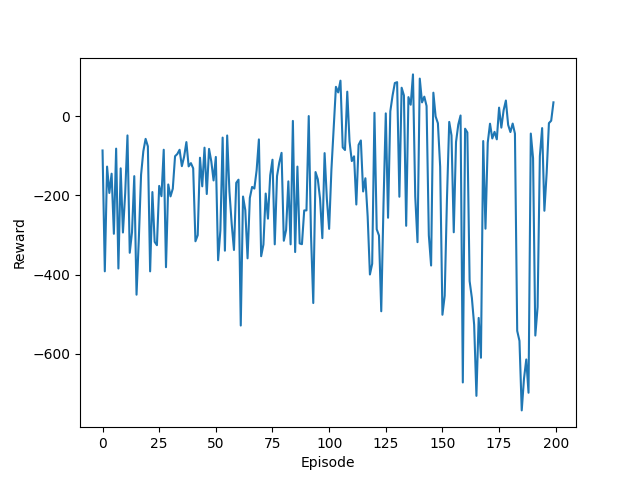
\includegraphics[scale=0.5]{RewardByEpisode}

\vspace{5mm}

This Deep Q learning model was not fully successful on the Lunar Lander problem - it does not seem like the model was able to learn the task fully, as rewards are not reaching very high levels (200 being the highest).
Nevertheless, performance significantly improved after modifying the network architecture, adding a customized reward function, and attempting to optimize the learning parameters to the greatest degree possible. While
the problem was not fully learned, the model has clearly been able to make progress, as seen in the plot charting rewards over time.

\end{document}
